\let\negmedspace\undefined
\let\negthickspace\undefined
\documentclass[journal]{IEEEtran}
\usepackage[a5paper, margin=10mm, onecolumn]{geometry}
%\usepackage{lmodern} % Ensure lmodern is loaded for pdflatex
\usepackage{tfrupee} % Include tfrupee package

\setlength{\headheight}{1cm} % Set the height of the header box
\setlength{\headsep}{0mm}     % Set the distance between the header box and the top of the text

\usepackage{gvv-book}
\usepackage{gvv}
\usepackage{cite}
\usepackage{amsmath,amssymb,amsfonts,amsthm}
\usepackage{algorithmic}
\usepackage{graphicx}
\usepackage{textcomp}
\usepackage{xcolor}
\usepackage{txfonts}
\usepackage{listings}
\usepackage{enumitem}
\usepackage{mathtools}
\usepackage{gensymb}
\usepackage{comment}
\usepackage[breaklinks=true]{hyperref}
\usepackage{tkz-euclide} 
\usepackage{listings}
% \usepackage{gvv}                                        
\def\inputGnumericTable{}                                 
\usepackage[latin1]{inputenc}                                
\usepackage{color}                                            
\usepackage{array}                                            
\usepackage{longtable}                                       
\usepackage{calc}                                             
\usepackage{multirow}                                         
\usepackage{hhline}                                           
\usepackage{ifthen}                                           
\usepackage{lscape}
\usepackage{circuitikz}
\tikzstyle{block} = [rectangle, draw, fill=blue!20, 
    text width=4em, text centered, rounded corners, minimum height=3em]
\tikzstyle{sum} = [draw, fill=blue!10, circle, minimum size=1cm, node distance=1.5cm]
\tikzstyle{input} = [coordinate]
\tikzstyle{output} = [coordinate]



\graphicspath{{figs/}}
\renewcommand{\theequation}{4.3.9.\arabic{equation}}
\renewcommand{\thefigure}{4.3.9.\arabic{figure}}

\bibliographystyle{IEEEtran}
\vspace{1.5em}

\title{4.3.9}
\author{E Achyuta Siddartha - ee25btech11024}

\begin{document}
\maketitle

\noindent
\textbf{Problem Statement} \\
The vector equation of the line
\begin{align}
\frac{x - 5}{3} = \frac{y + 4}{7} = \frac{z - 6}{2}
\label{eq:given}
\end{align}
is \_\_\_\_\_\_\_\_\_\_\_\_\_.

\vspace{1.5em}

\noindent
\textbf{Solution:} \\

From \eqref{eq:given} we get the following equations.
\begin{align}
    x &= 5 + 3\kappa, \label{eq:a} \\ 
    y &= -4 + 7\kappa, \label{eq:b} \\ 
    z &= 6 + 2\kappa. \label{eq:c}
\end{align}

The general vector equation of a line in 3D is
\begin{align}
\vec{x} = \vec{h} + \kappa \vec{m},   
\label{eq:formula}
\end{align}

comparing \eqref{eq:a}, \eqref{eq:b}, \eqref{eq:c}, and \eqref{eq:formula} we get,
\begin{align}
\vec{h} = \myvec{5 \\ -4 \\ 6}, \quad 
\vec{m} = \myvec{3 \\ 7 \\ 2}.    
\end{align}


\noindent
\textbf{Therefore, the vector equation of the line is:}
\begin{align}
\vec{x} = \myvec{5 \\ -4 \\ 6} + \kappa \myvec{3 \\ 7 \\ 2}
\end{align}


See Figure~\ref{fig:line3D}.

\begin{figure}[h!]
    \centering
    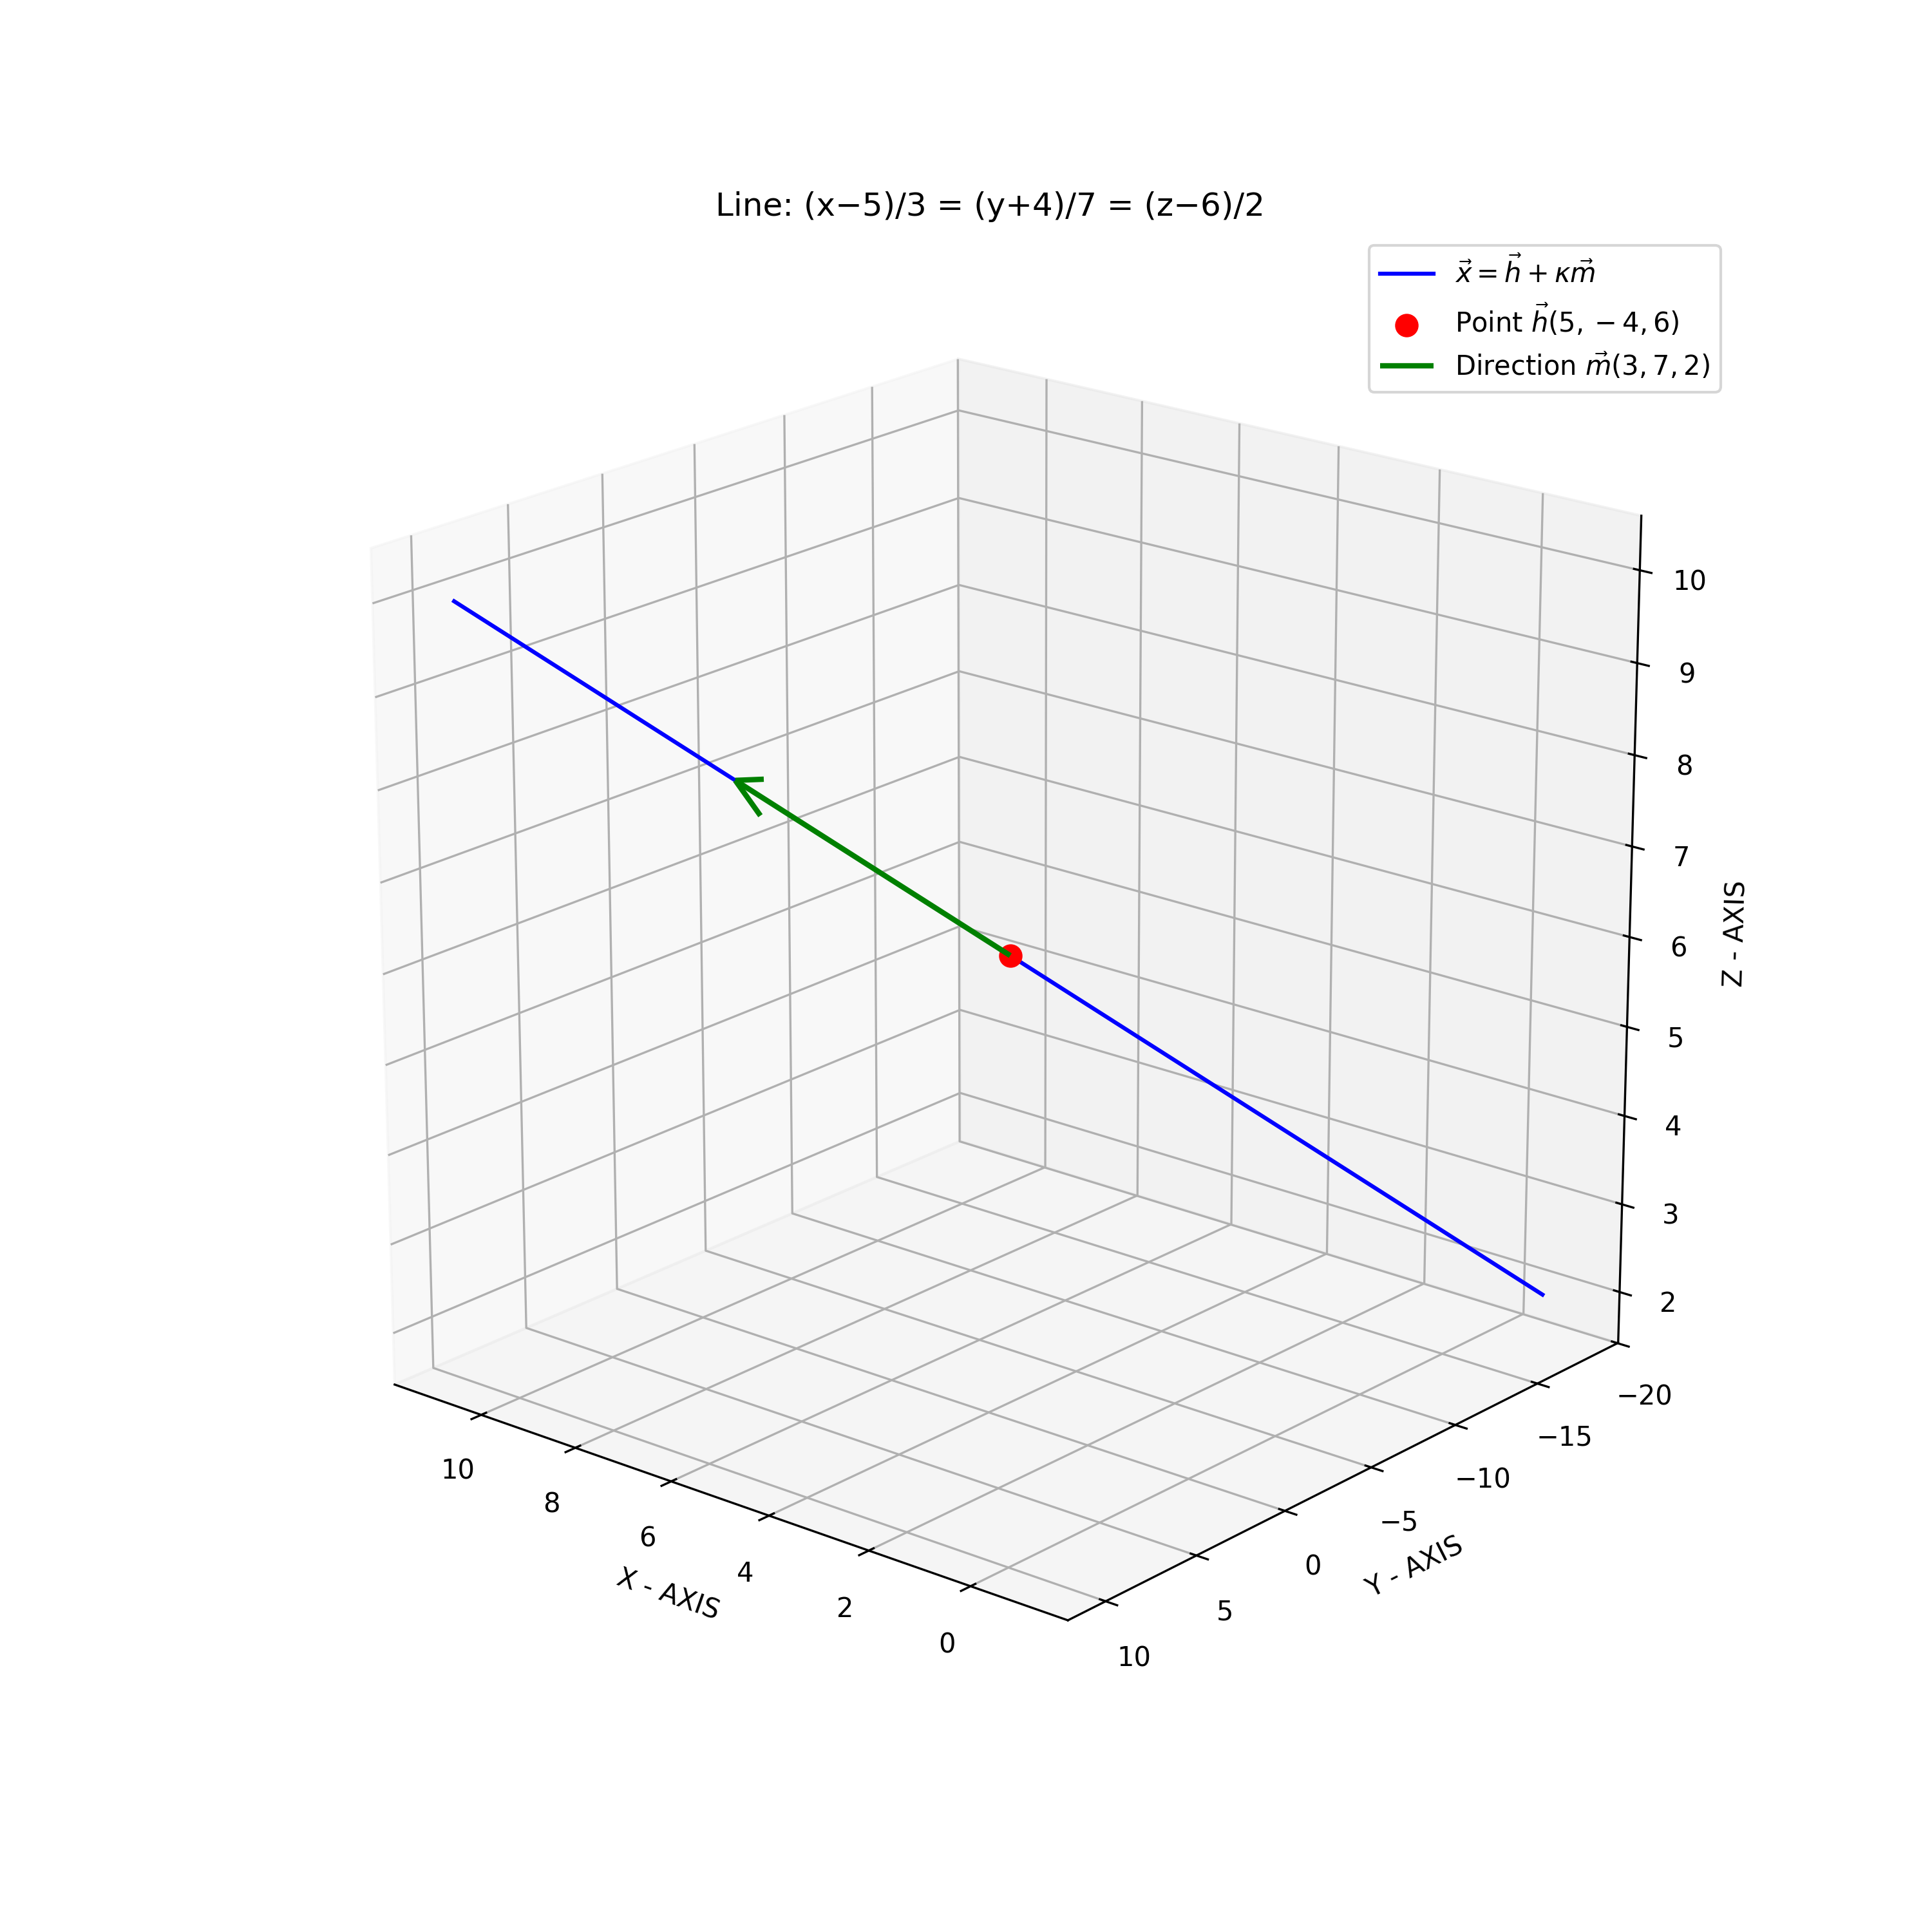
\includegraphics[width=1.0\linewidth]{figs/fig.png}
    \caption{}
    \label{fig:line3D}
\end{figure}


\end{document}